\documentclass{standalone}
\usepackage{tikz}
\begin{document}

			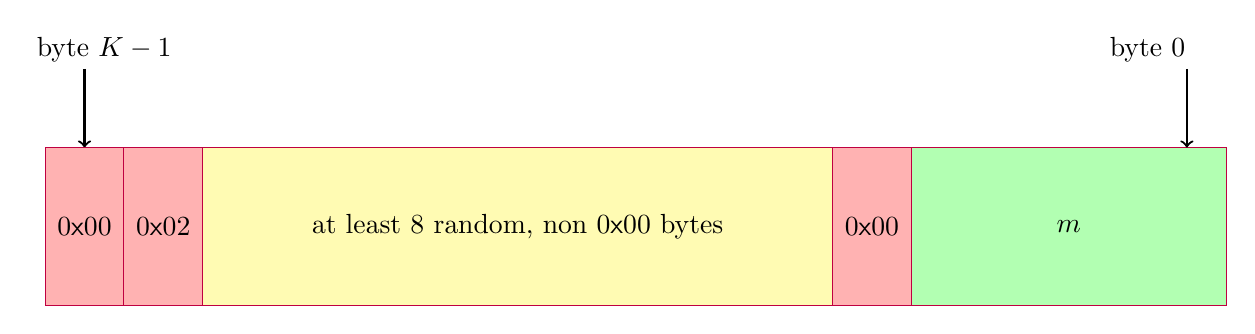
\begin{tikzpicture}
				\node [] at (0.75,3.25) {byte $K-1$};
				\draw[->,thick] (0.5,3) -- (0.5,2);
				\draw [fill=red!30,draw=purple] (0,0) rectangle (1,2);
				\node [] at (0.5,1) {$0\mathsf{x}00$};
				\draw [fill=red!30,draw=purple] (1,0) rectangle (2,2);
				\node [] at (1.5,1) {$0\mathsf{x}02$};
				\draw [fill=yellow!30,draw=purple] (2,0) rectangle (10,2);
				\node [] at (6,1) {at least $8$ random, non $0\mathsf{x}00$ bytes};
				\draw [fill=red!30,draw=purple] (10,0) rectangle (11,2);
				\node [] at (10.5,1) {$0\mathsf{x}00$};
				\draw [fill=green!30,draw=purple] (11,0) rectangle (15,2);
				\node [] at (13,1) {$m$};
%				\draw [fill=green!30,draw=purple] (14,0) rectangle (15,2);
				\node [] at (14,3.25) {byte $0$};
				\draw[->,thick] (14.5,3) -- (14.5,2);
			\end{tikzpicture}	
\end{document}
